The purpose of this case is to test the calculation of exceedance curves for occupant fatalities for an asset. The number of occupants for the asset used in this case are 2 (day), 4 (transit), and 6 (night). An average value of 4 occupants is used for the calculation of the exceedance curve and average annual fatalities. Table~\ref{tab:vf-ln-tax1-dnt} shows the mean loss ratios and corresponding coefficients of variation for the occupants fatality vulnerability function used in this test case. Apart from the change in the vulnerability function and value, the calculation procedure remains the same as described in Case~1d.

% The loss curve calculated using the implementation of the calculator in Julia is compared with that produced by OpenQuake in Figure~\ref{fig:lc-ebr-2d}.

% \begin{figure}[htbp]
% \centering
% 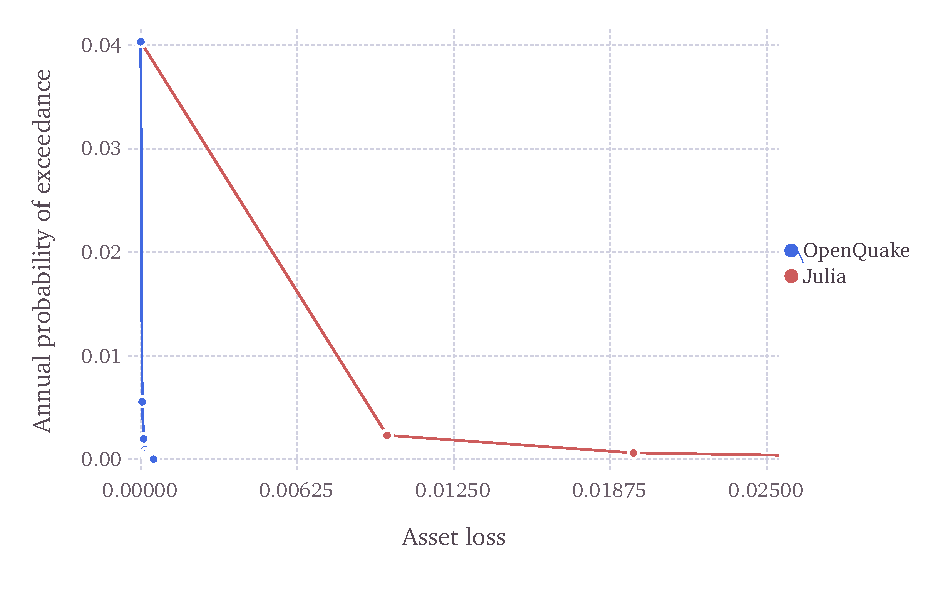
\includegraphics[width=12cm]{qareport/figures/fig-lc-ebr-2d}
% \caption{Loss curve comparison for event based risk test case 2d}
% \label{fig:lc-ebr-2d}
% \end{figure}